\chapter{Test af det samlede system}
\label{bilag:test}
Testens formål er at udføre en vector network analyse af det samlede system for at finde systemets amplitude-karakteristik. 
Det samlede system består af modtageren af indgangssignalet, anti-aliasing filtrene for den ene kanal, Tiva-kittet med EMP board og microcontroller, DAC, rekonstruktionsfilteret for den ene kanal og udgangskredsløbet. 

\subsection{Udstyr}
\begin{itemize}
	\item Bode 100 med tilhørende udstyr
	\item Èn computer med Bode Analyzer Suite installeret
	\item To oscilloskop-prober
	\item Skillekondensator
\end{itemize}

\subsection{Fremgangsmåde og forsøgsopstilling}
Opsæt Bode 100 uden noget tilsluttet. 
Åben Bode Analyzer Suite, og vælg en Gain/Phase-analyse under Vector Network Analysis. 
Analysen sættes op med følgende indstillinger:
\begin{multicols}{2}
\begin{itemize}
	\item Startfrekvens: 10 Hz
	\item Slutfrekvens: 50 kHz
	\item Minimum 401 data points
	\item Source level: 0 dBm
	\item Attenuator på receiver 1 \& 2: 10 dB
	\item Receiver bandwidth: 100 Hz
	\item External reference på CH1 \& CH2
\end{itemize}
\end{multicols}
Vælg Trace 1 til Magnitude (dB). \newline
Med Bode Analyzer suite laves en kalibrering af Bode 100, når udgangen og indgangene på Bode 100 er koblet sammen. 
Skillekondensatoren skal være på udgangen. \newline
Opsæt det samlede system som vist på figur \ref{fig:lol}. 
Bode 100's udgang med skillekondensator og CH1 kobles til indgangen på den ene kanal af det samlede system. 
CH2 kobles til udgangen af det samlede system for den tilsvarende kanal. 
Analysen kan nu udføres. 

\subsection{Resultat af test}
Datasættet for resultatet af testen kan ses i den vedhæftede fil \textit{'habibi.csv'}. 
\husk{Jes}{Filnavn skal rettes her!}
\begin{figure}[h]
	\caption{Overføringsfunktionen af det samlede system.}
	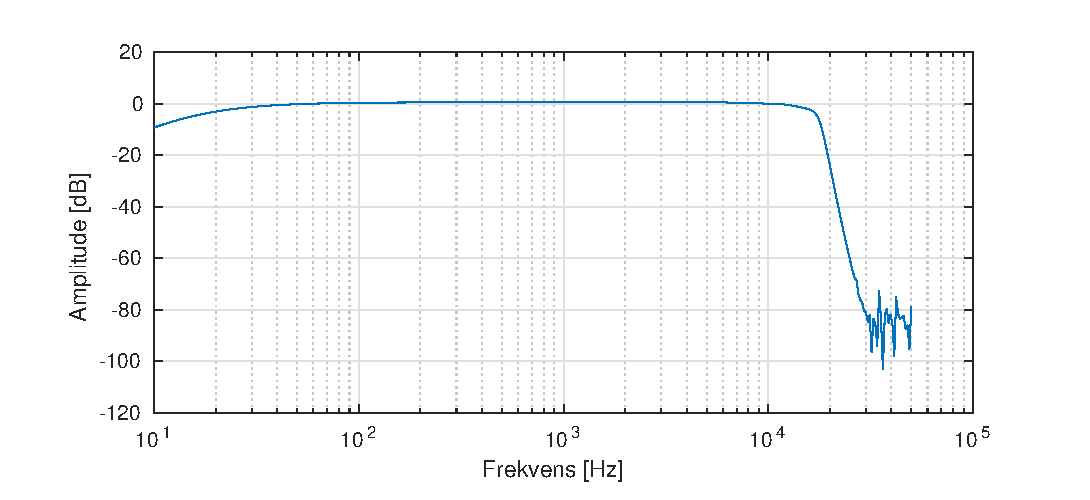
\includegraphics[width=1\linewidth]{./billeder/tf_samletsystem.eps}
	\label{fig:tf_samletsystem}
\end{figure}

\section{Test af anti-aliasing filtre}
%Formål her.
Testen følger samme fremgangsmåde, som ved testen af det samlede system. 
Dog testes udelukkende anti-aliasing filtrene. 